\chapter{AWS Amplify}

Das folgende Kapitel beschreibt die Architektur und die Implementierung mit Amplify.

\section{Architektur}

\subsection{Lösungsstrategie}

Die Architektur folgt dem Aufbau einer Drei"=Schichten"=Architektur:

\begin{itemize}
  \item Präsentationsschicht
    \begin{itemize}
      \item React.js
      \item amplify-js
    \end{itemize}
  \item Logikschicht
    \begin{itemize}
      \item AppSync
      \item Lambda
      \item Cognito
      \item Elemental MediaConvert
      \item EventBridge
      \item IAM
    \end{itemize}
  \item Datenhaltungsschicht
    \begin{itemize}
      \item DynamoDB
      \item S3
      \item Cognito
      \item IAM
      \item AWS Backup
    \end{itemize}
\end{itemize}

Die Cloud-Dienste Cognito und IAM befindet sich zugleich in zwei Schichten, da dort neben der Logik für Authentifizierung und Autorisierung auch die Benutzer persistiert werden.

Durch die ausschließliche Verwendung interner Cloud-Dienste, keiner Eigenentwicklungen für die Benutzerverwaltung und definierter Technologien sind die Rahmenbedingungen für dieses Projekt nicht missachtet, so dass die Vergleichbarkeit weiterhin gegeben ist.

\autoref{Kap2:Teildisziplinen} zeigt erste Lösungsansätze, um die nichtfunktionalen Anforderungen, auch Qualitätsziele genannt, zu erreichen.

\begin{table}[h]
  \caption{Lösungsansatz für nichtfunktionale Anforderungen}
  \label{Kap2:Teildisziplinen}
  \renewcommand{\arraystretch}{1.2}
  \centering
  \sffamily
  \begin{footnotesize}
    \begin{tabularx}{0.9\textwidth}{l l X}
      \toprule
      \textbf{Anforderung} & \textbf{Dienst} & \textbf{Ansatz}\\
      \midrule
        \emph{Verfügbarkeit} & Amplify & Amplify bietet für Frontend und Backend ein Zero-Downtime Deployment. \\
        \emph{Skalierbarkeit} & - & Durch die Serverless-Architektur skalieren Dienste automatisch innerhalb der \ac{AWS}-Cloud.\\
        \emph{Analysierbarkeit} & CloudWatch & Durch den Einsatz von CloudWatch können Anfragen für jeden Cloud-Dienst nachvollzogen werden.\\
        \emph{Interoperabilität} & AppSync & Durch den Einsatz von AppSync ist mit GraphQL eine einheitliche Schnittstelle sichergestellt.\\
        \emph{Backups} & AWS Backup & Durch den Einsatz von AWS Backup werden automatisiert Backups aufgesetzt.\\
        \emph{Wiederherstellbarkeit} & AWS Backup &  Das von AWS Backup erstellte Backup für die Datenbank DynamoDB kann manuell eingespielt werden.\\
      \bottomrule
    \end{tabularx}
  \end{footnotesize}
  \rmfamily
\end{table}

\subsection{Bausteinsicht}

Beschreibung der Ressource die benötigt werden, welcher Service dahinter steht und was dieser macht, ggf. als Liste. Gruppierung in Form von Stacks (IaaS), so dass das Deployment später einfach beschrieben werden kann

RootStack:
...

ApiStack:
  - API: AppSync
  - AWS::AppSync::GraphQLApi
  - AWS::AppSync::GraphQLSchema
  - AWS::AppSync::Resolver (ggf. über weitere unterstacks)
  - AWS::AppSync::DataSource (ggf. über weitere unterstacks)
  - AWS::DynamoDB::Table

AuthStack:
  - AWS::Cognito::IdentityPool
  - AWS::Cognito::IdentityPoolRoleAttachment
  - AWS::IAM::Role
  - AWS::Cognito::UserPool
  - AWS::Cognito::UserPoolClient
  - Custom::LambdaCallout
  - AWS::Lambda::Function
  - AWS::IAM::Policy

AuthUserPoolGroupStack:
  - AWS::Cognito::UserPoolGroup
  - AWS::IAM::Role
  - AWS::Lambda::Function
  - Custom::LambdaCallout

StorageStack:
  - AWS::S3::Bucket
  - AWS::IAM::Policy

FunctionLayerStack:
  - AWS::Lambda::LambdaLayerVersion, AWS::Lambda::LayerVersionPermission

FunctionCreateVideoStack:
  - AWS::IAM::Policy, AWS::IAM::Role, AWS::Lambda::Function, AWS::MediaConvert::JobTemplate, AWS::MediaConvert::Queue

FunctionVideoConvertedStack:
- AWS::Events::Rule, AWS::Lambda::Permission, AWS::IAM::Role, AWS::Lambda::Function, AWS::IAM::Policy

FunctionCreateLinkStack:
- AWS::IAM::Role
- AWS::Lambda::Function
- AWS::IAM::Policy

- Storage: S3-Bucket
- Lambda:
  - CreateVideo
  - CreateLink
  - VideoConverted
- DB: DynamoDB
- Job: MediaConvert
- EventBridge

\subsection{Laufzeitsicht}

todo text

\subsubsection{Lesen, Aktualisieren und Löschen eines Videos}

Der folgende Prozess beschreibt, wie Videos von Nutzern gelesen, aktualisiert oder gelöscht werden.

\begin{figure}
  \centering
  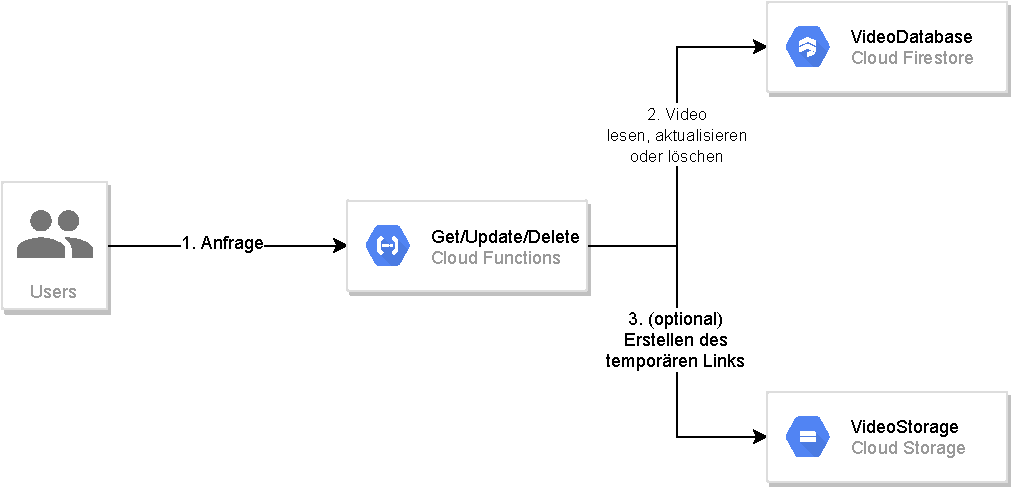
\includegraphics[width=0.75\columnwidth]{5_aws-amplify/laufzeitsicht_1.pdf}
  \caption{AWS Amplify - Laufzeitsicht - Lesen, Aktualisieren und Löschen eines Videos}
  \label{Amplify:laufzeitsicht1}
\end{figure}

\subsubsection{Erstellen eines Videos}

Der nächste Prozess beschreibt den Ablauf, wie ein Video von einem Nutzer erstellt wird.

\begin{figure}
  \centering
  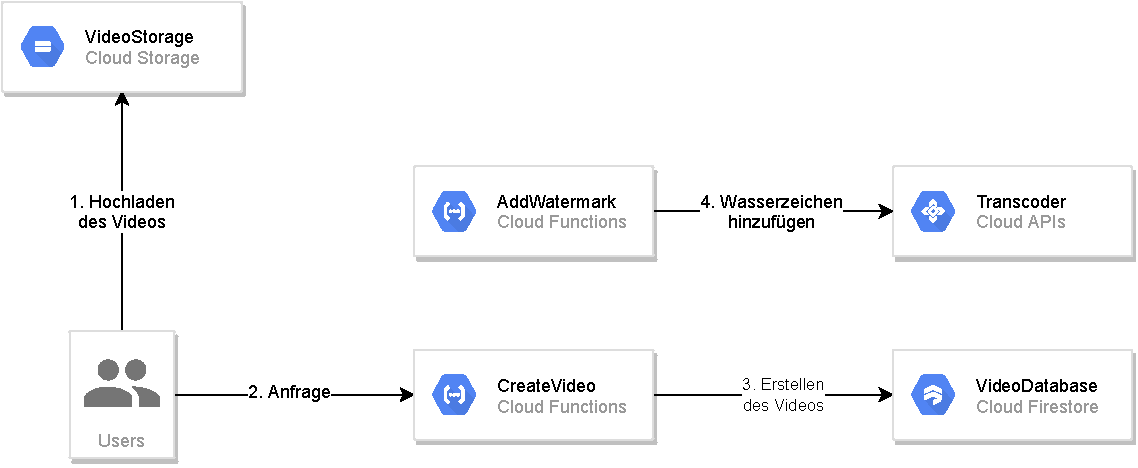
\includegraphics[width=1\columnwidth]{5_aws-amplify/laufzeitsicht_2.pdf}
  \caption{AWS Amplify - Laufzeitsicht - Erstellen eines Videos}
  \label{Amplify:laufzeitsicht2}
\end{figure}

\subsubsection{Erstellen von signierten Links}

Dieser Prozess beschreibt, wie Nutzer signierte temporäre Links erstellen können, um das Video anzuzeigen.

\begin{figure}
  \centering
  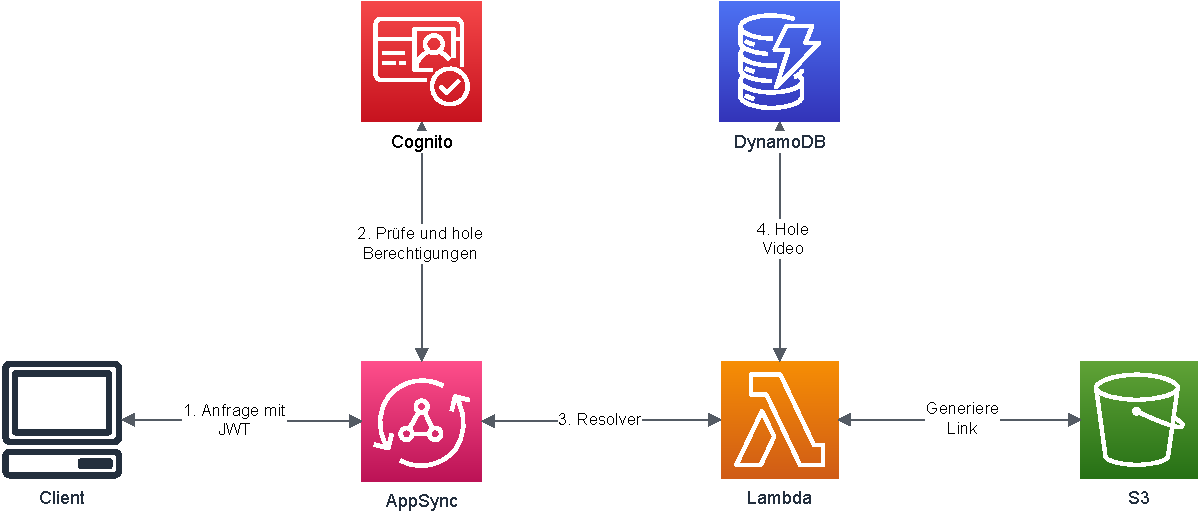
\includegraphics[width=1\columnwidth]{5_aws-amplify/laufzeitsicht_3.pdf}
  \caption{AWS Amplify - Laufzeitsicht - Erstellen von Links}
  \label{Amplify:laufzeitsicht3}
\end{figure}

\subsection{Verteilungssicht}

\begin{figure}
  \centering
  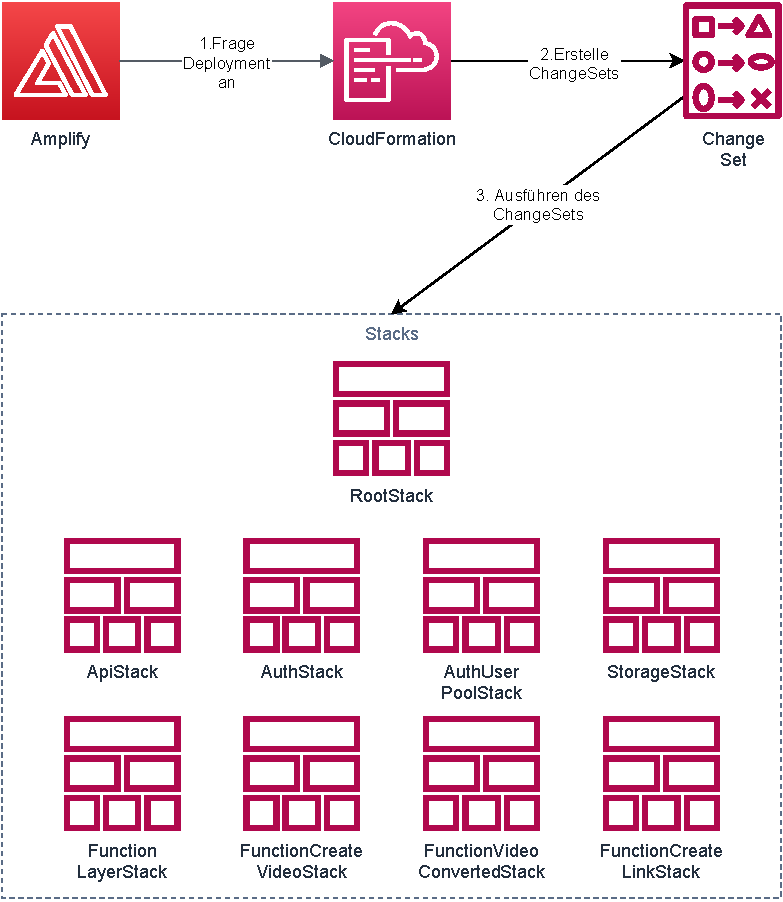
\includegraphics[width=0.75\columnwidth]{5_aws-amplify/verteilungssicht.pdf}
  \caption{AWS Amplify - Verteilungssicht}
  \label{Amplify:verteilungssicht}
\end{figure}

Einordnung der Bausteinsicht-Elemente in Stacks für Verteilung

Es gibt keine Substacks, aber weitere parentstacks - das ist vermutlich für die Debuggbarkeit.

\subsection{Querschnittliche Konzepte und Muster}

- Einbindung über \ac{AWS} Amplify:
  - AWS Elemental MediaConvert als extra Plugin
  - Anpassung an CF-Templates
- Logging (CloudWatch)
- Permissions (IAM)
- AWS Backup

\subsection{Entwurfsentscheidungen}

\subsection{Risiken und technische Schulden}

- Auth: Anpassung, dass statt Identity ID die Pool User Id genutzt wird geht über https://github.com/aws-amplify/amplify-js/issues/54. Leider lässt sich das nicht persistieren, so dass man das bei jedem branch/Projekt neu eintragen muss. Wenn man es im CF-Template ändert, wird die Änderung beim Push rückgängig gemacht. Das ist nicht sehr flexibel. Ggf. Lösung finden und schauen, ob es doch geht.

- CDK als Alternative zu AWS Amplify, da es wesentlich flexibler

\section{Implementierung}